\subsection{Feed-Forward: Asymmetry and Mixed Interactions}\label{sec:ffresults}\label{sec:ffinteractionresults}

The new cohort separates the nonce-word asymmetry of the working state from its change under finalization. At two rounds and 128-bit resolution, Salsa20 has $G_{\rm none}=+0.72940$ bits and $G_{\rm add}=+0.78805$ bits. The planned paired increase is $+0.05865$ bits [$+0.05535$, $+0.06202$]. Both planned endpoints reach the four-test Holm simulation floor (Table~\ref{tab:fftests}). The asymmetry therefore precedes feed-forward. Supplementary Table S5 lists all three finalizations and their intervals, including $G_{\rm xor}=+0.73896$ bits for Salsa20/2.

The planned ChaCha20 add-minus-none change at 128 bits is $-0.00293$ bits [$-0.00652$, $+0.00068$], with Holm-adjusted $p=0.108$. This unresolved endpoint is specific to the selected resolution. Descriptively, the corresponding changes at 32 and 64 bits are $-0.02289$ and $-0.00772$ bits, with pointwise intervals excluding zero. Salsa20's gap is positive under every intervention at all three widths, and its add-minus-none changes at 32 and 64 bits are $+0.04962$ and $+0.04641$ bits. 

\begin{table}[H]
\caption{The four planned endpoints of the paired feed-forward experiment, all at two rounds on the same 80 key pairs. $E_1$--$E_3$ use 128-bit segments and are entropy differences in bits. $E_4$ is the interaction contrast $J$ of Equation~\eqref{eq:ffinteraction}, measured in changed bits per 32-bit output word. Intervals are pointwise 95\% whole-key bootstrap intervals; all four two-sided tests share one Holm family. The value $4.0\times10^{-5}$ is the simulation floor after correction.\label{tab:fftests}}
\footnotesize\setlength{\tabcolsep}{3pt}
\begin{tabularx}{\textwidth}{lXCC}
\toprule
\textbf{Test} & \textbf{Endpoint} & \textbf{Mean [95\% CI]} & \textbf{Holm $p$}\\
\midrule
$E_1$ & Salsa20 $G_{\rm none}$ & \shortstack{$+0.72940$\\$[+0.72392,+0.73493]$} & $4.0\times10^{-5}$\\
\addlinespace[3pt]
$E_2$ & Salsa20 $G_{\rm add}-G_{\rm none}$ & \shortstack{$+0.05865$\\$[+0.05535,+0.06202]$} & $4.0\times10^{-5}$\\
\addlinespace[3pt]
$E_3$ & ChaCha20 $G_{\rm add}-G_{\rm none}$ & \shortstack{$-0.00293$\\$[-0.00652,+0.00068]$} & $0.108$\\
\addlinespace[3pt]
$E_4$ & Salsa20 mixed word-7 interaction $J$ & \shortstack{$+0.70967$\\$[+0.68263,+0.73686]$} & $4.0\times10^{-5}$\\
\bottomrule
\end{tabularx}
\end{table}

\paragraph{Mixed nonce interactions.}

For Salsa20/2 output word 7, the mean derivative HW over the 31 aligned non-MSB cross-word pairs is exactly zero under none and xor, and $0.72419$ changed bits under add. Subtracting the paired reference change gives the planned $J=+0.70967$ [$+0.68263$, $+0.73686$], which reaches the adjusted simulation floor. The reference means are close to 16 changed bits under each intervention. This paired effect does not bring the response close to the reference level of 16 bits.

The complete profiles in Figure~\ref{fig:ffderivatives} show effects beyond the selected word. For example, Salsa20 word 11 has a descriptive mean of zero before feed-forward and approximately 1.154 changed bits after modular addition. ChaCha20 word 7 already has a mean of 8.73687 changed bits before feed-forward, rising to 10.93961 under add. The exact zero followed by a nonzero mixed response is therefore a statement about particular Salsa20 output dependencies, while modular finalization also changes responses elsewhere.

\begin{figure}[!t]
\centering
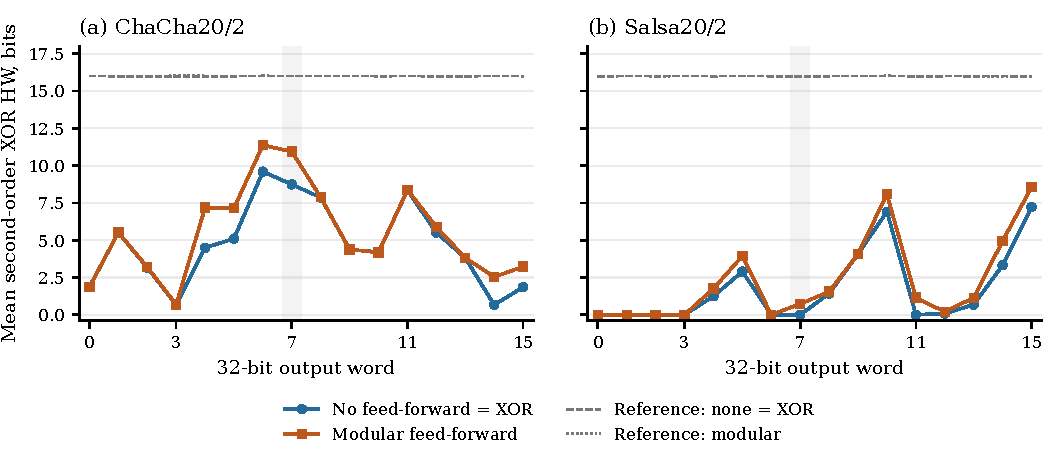
\includegraphics[width=\textwidth]{publication_feedforward_derivatives}
\caption{Mean HW of the second-order output derivative for (a) ChaCha20/2 and (b) Salsa20/2, averaged within each key over the 31 aligned cross-word bit offsets 0--30, four base nonces, and 16 output blocks. Values are raw means for each 32-bit word, rather than cipher-minus-reference contrasts. None and xor share one curve because their derivatives agree bit for bit; the separate add curve uses standard modular feed-forward. Gray lines show the coupled reference means. Shaded bands are pointwise 95\% whole-key bootstrap intervals from 5000 paired resamples of the 80 key pairs. The highlighted position is output word 7, used in the planned Salsa20 interaction endpoint. Other output positions are descriptive.\label{fig:ffderivatives}}
\end{figure}

All algebraic checks pass. None and xor derivatives agree in all 12,451,840 cipher word comparisons and the same number of reference comparisons, across both cores and both round counts. For Salsa20/2, the conditional $L_b(C)$ formula matches all 184,320 mixed add derivatives, including the offset panel. In this two-round Salsa20 setting, the cipher derivatives for both within-second-word control pairs are zero in word 7 under every intervention, and the bit-31 cancellations and singleton identities also have no violations. These are deterministic checks, not additional statistical replicates.

At four rounds, the largest absolute mean nonce-word gap across both cores, all three interventions, and all three widths is 0.00142 bits. Some small pointwise gap intervals exclude zero. The descriptive interaction contrasts are $J=+0.00130$ [$-0.02630$, $+0.02775$] for ChaCha20 and $+0.02033$ [$-0.00832$, $+0.04826$] for Salsa20. These smaller contrasts do not establish equivalence to the reference.
